\appendix

\chapter{Rotating spin Hamiltonian}\label{app:rotating_spin_hamiltonian}

In Chap.~\ref{chap:2_adiabaticity} we used the example of a spin rotating in a magnetic field to illustrate adiabatic processes in quantum systems. We considered a spin starting in the $\ket{+}$ state and being rotated from the $x$ direction to the $z$ direction during some total time $\tau$ according to the Hamiltonian in Eq.~\eqref{eq:rotating_spin_H}, which I will reproduce here for convenience:
\begin{equation}\label{eq:rotating_spin_H_lambda_2}
    H(\lambda) = -\cos(\lambda)\sx - \sin(\lambda)\sz,
\end{equation}
with $\lambda(t) = \frac{\pi t}{2 \tau}$. The \acrref{AGP} operator ansatz $\approxAGP$ for this system can be described by the operator $\sy$ scaled by some $\lambda$-dependent coefficient which we will refer to as $\alpha(\lambda)$
\begin{equation}
    \approxAGP = \alpha(\lambda) \sy
\end{equation}
as discussed in the main text. We will now proceed to show how we can arrive at the resulting form of $\alpha$ given in Eq.~\eqref{eq:rotating_spin_alpha} using the \acrref{LCD} method outlined in Sec.~\ref{sec:2.4.1_LCD}.

The first step is to find the operator $G_{\lambda}$ given in Eq.~\eqref{eq:G_operator}:
\begin{equation}
    \begin{aligned}
        G_{\lambda}(\approxAGP) &= \dlambda H + i\comm{\approxAGP}{H} \\
        & = \sin(\lambda)\sx - \cos(\lambda)\sz + 2\alpha(\lambda)\sin(\lambda)\sx - 2\alpha(\lambda) \cos(\lambda)\sz \\
        & = (1 + 2\alpha(\lambda))\sin(\lambda) \sx - (1 + 2\alpha(\lambda))\cos(\lambda)\sz,
    \end{aligned}
\end{equation}
where we have used $\hbar = 1$. This can then be used to define the action
\begin{equation}
    \begin{aligned}
        \mathcal{S}(\approxAGP) &= \Tr\left[G^2_{\lambda}(\approxAGP) \right] \\
        & = 2 (1 + 2\alpha(\lambda))^2 \sin^2(\lambda) + 2 (1 + 2\alpha(\lambda))^2 \cos^2(\lambda) \\
        & = 2 (1 + 2\alpha(\lambda))^2.
    \end{aligned}
\end{equation}
In order to find the form of $\alpha$, we need to find the minimum of the action $\mathcal{S}(\approxAGP)$ with respect to $\alpha$, which can be easily done:
\begin{equation}
    \begin{aligned}
        \frac{\delta \mathcal{S}}{\delta \alpha} &= 8(1 + 2\alpha(\lambda)) \\
        \Rightarrow \alpha(\lambda) &= -\frac{1}{2},
    \end{aligned}
\end{equation}
which is the expected result. 

It can be checked, for this simple example, that $\approxAGP = -\frac{1}{2} \sy$ is the exact \acrref{AGP} operator $\AGP{\lambda}$ by using Eq.~\eqref{eq:AGP_adiabatic_basis} where the matrix elements of the \acrref{AGP} are written out explicitly as:
\begin{equation}
    \begin{aligned}
        \AGP{\lambda} &= i \Big(\sum_n \braket{n}{\dlambda n} \dyad{n} + \sum_{m \neq n} \ket{m} \frac{\mel{m}{\dlambda H}{n}}{(E_n - E_m)} \bra{n} \Big) \\
        & = i \Big(\sum_n \braket{n}{\dlambda n} \dyad{n} + \sum_{m \neq n} \braket{m}{\dlambda n} \dyad{m}{n}\Big)
    \end{aligned}
\end{equation}

In this case, the adiabatic eigenstates of the Hamiltonian $H(\lambda)$ are
\begin{equation}
    \begin{aligned}
        \ket{\psi_1} &= \frac{1}{n_1} \left[(\sec(\lambda) + \tan(\lambda)) \ket{\uparrow} + \ket{\downarrow}\right] \\
        \ket{\psi_2} &= \frac{1}{n_2} \left[(-\sec(\lambda) + \tan(\lambda)) \ket{\uparrow} + \ket{\downarrow}\right],
    \end{aligned}
\end{equation}
where $n_1 = \sqrt{1 + \abs{\sec(\lambda) + \tan(\lambda)}^2}$ and $n_2 = \sqrt{1 + \abs{-\sec(\lambda) + \tan(\lambda)}^2}$ are the normalisation factors. Their derivatives with respect to $\lambda$ are
\begin{equation}
    \begin{aligned}
        \ket{\dlambda \psi_1} &= \frac{1}{n_1^3} \sec(\lambda) \left[(\sec(\lambda) + \tan(\lambda))\ket{\uparrow}  - (\sec(\lambda) + \tan(\lambda))^2 \ket{\downarrow}\right] \\
        \ket{\dlambda \psi_2} &= (2 + 2\sin(\lambda))^{-3/2} \left[(\sin(\lambda) + 1)^2 \ket{\uparrow} + \cos(\lambda)(1 + \sin(\lambda))\ket{\downarrow}\right].
    \end{aligned}
\end{equation}

Evaluating $\braket{\psi_1}{\dlambda \psi_1}$ and $\braket{\psi_2}{\dlambda \psi_2}$ we find that they are equal to $0$, meaning the diagonal elements of $\AGP{\lambda}$ are $0$. Doing the same for the off-diagonals we find 
\begin{equation}
    \begin{aligned}
        \braket{\psi_1}{\dlambda \psi_2} &= \frac{1}{2} \\
        \braket{\psi_2}{\dlambda \psi_1} &= -\frac{1}{2},
    \end{aligned}
\end{equation}
meaning that the exact \acrref{AGP} operator, as found from evaluating its matrix elements is just
\begin{equation}
    \AGP{\lambda} = \mqty(0 & \frac{i}{2} \\ -\frac{i}{2} & 0) = \alpha(\lambda) \sy,
\end{equation}
which is the result obtained previously from the \acrref{LCD} approach. 

\chapter{Pontryagin maximum principle}\label{app:PMP}

This part of the appendix is dedicated solely to introducing the Pontryagin maximum principle or \acrref{PMP}, which, while not used in the main results of the thesis, forms the backbone of analytical optimal control theory, which I discuss at length in Ch.~\ref{chap:3_Quantum_Optimal_control}. In formal terms, the \acrref{PMP} can be defined \cite{dalessandro_introduction_2021} by the following theorem.

\newtheorem{theorem}{Theorem}

\begin{theorem}[\acrref{PMP} for Mayer problems]\label{thm:pmp}
    For fixed final time $\tau$ and free final state assume $u$ is the optimal control and $x$ the corresponding trajectory solution of Eq.~\eqref{eq:control_ODE}. Then, there exists a nonzero vector $\lambda$ solution of the adjoint equations
  \begin{equation}
      \dotlambda^T = - \lambda^T f(x(t), u(t))
  \end{equation}
  with terminal condition
  \begin{equation}
      \lambda^T(\tau) = -\phi(x(\tau))
  \end{equation}
  such that, for almost every $t \in (0, \tau]$, we have
  \begin{equation}\label{eq:pmp_maximisation}
      \lambda^T(t) f(x(t), u(t)) \geq \lambda^T(t) f(x(t), v)
  \end{equation}
  for every $v$ in the set of the admissible values for the control $U$. Furthermore, for every $t \in [0, \tau]$
  \begin{equation}\label{eq:pmp_constant}
      \lambda^T(t) f(x(t), u(t)) = c,
  \end{equation}
  for a constant $c$
\end{theorem}

Using this, one can then define the \emph{optimal control Hamiltonian}:
\begin{equation}
    h(\lambda, x, u) := \lambda^T(t) f(x, u).
\end{equation}
Now we can recast Eqs.~\eqref{eq:pmp_maximisation} and \eqref{eq:pmp_constant}:
\begin{equation}
    \begin{aligned}
        h(\lambda(t), x(t), u(t)) &= c \\
        h(\lambda, x, u) &\geq h(\lambda, x, v),
    \end{aligned}
\end{equation}
The solution will be of the form $u := u(x, \lambda)$ and it can be solved with the system of equations
\begin{equation}
    \begin{aligned}
        \dot{x} &= f(x, u(x, \lambda)), \\
        \dotlambda^T &= -\lambda^T f(x, u(x, \lambda))
    \end{aligned}
\end{equation}
with the boundary conditions $x(0) = x_0$ and $\lambda^T(\tau) = -\phi(x(\tau))$. Every control which is obtained with this procedure satisfies the necessary conditions of optimality and it is a candidate to be the optimal control.

\chapter{Derivation of the CD coefficients for an arbitrary Ising graph}\label{app:arbitrary_ising_derivation}

In the main text, we discuss deriving the local counterdiabatic driving or \acrref{LCD} terms to first and second order for an Ising graph of $N$ spins with arbitrary couplings between them. In this appendix, we will show a full derivation for the coupled set of equations required to determine the coefficients for said terms.

An Ising Hamiltonian for $N$ spins and with both a transverse and longitudinal field and with arbitrary couplings can be written as:
\begin{equation}\label{eq:ising_hamiltonian}
    H(\lambda) = \sum_{i = 1}^{N-1}\sum_{j = i+1}^{N} J_{ij}(\lambda) \sz_i \sz_j + \sum_{i = 1}^{N} \Big( X_i(\lambda) \sx_i + Z_i(\lambda) \sz_i \Big)
\end{equation}
where the coefficients $J_{ij}$ correspond to couplings between spins $i$ and $j$. Systems like this can be viewed as undirected graphs, with each spin corresponding to a vertex and each coupling $J_{ij}$ denoting an edge between the corresponding spins. In the case of a weighted graph, the magnitude of each $J_{ij}$ can be viewed as the weight of the corresponding edge. This type of Hamiltonian, for specific values of $J_{ij}$, $X_i$ and $Z_i$ can be used to describe the two-spin annealing example of Sec.~\ref{sec:5.1_2spin_annealing}, the Ising chain from Sec.~\ref{sec:5.2_Ising_chain} and the frustrated spin model of Sec.~\ref{sec:6.4_ghz_states}. 

The first order \acrref{LCD} ansatz, as stated in the main text, is just single-spin operators:
\begin{equation}\label{eq:spin_agp_1storder}
    \AGP{\lambda}^{(1)} = \sum_{i = 1}^N \alpha_i(\lambda) \sy_i
\end{equation}
and the second order can be split up into 4 separate symmetries of operators:
\begin{equation}\label{eq:spin_agp_2ndorder}
        \AGP{\lambda}^{(2)} = \sum_{i = 1}^{N-1}\sum_{j = i+1}^{N} \Big( \gamma_{ij}(\lambda) \sx_i \sy_j + \Bar{\gamma}_{ij}(\lambda) \sy_i \sx_j + \zeta_{ij}(\lambda) \sz_i \sy_j + \Bar{\zeta}_{ij}(\lambda) \sy_i \sz_j \Big).
\end{equation}

The first order commutators are computed as follows:
\begin{equation}\label{eq:first_order_AGP_commutator}
        i\comm{\alpha_i \sy_i}{H} = 2\alpha_i \Big[ \sum_{j = i+1}^{N} - J_{ij} \Big( \sx_i \sz_j + \sz_i \sx_j \Big) + X_i \sz_i - Z_i \sx_i \Big],
\end{equation}
where I have omitted the dependence on $\lambda$ of the terms. The second order expansions, sadly, look like this:
\begin{equation}
    \begin{aligned}
        i\comm{\gamma_{ij} \sx_i \sy_j}{H(\lambda)} &= 2\gamma_{ij} \Big[ \sum_{k = 1}^{i-1} (J_{ki} \sz_k \sy_i \sy_j - J_{kj} \sz_k \sx_i \sx_j)  + \sum_{k = i + 1}^{j-1} (J_{ik} \sy_i \sz_k \sy_j - J_{kj} \sx_i \sz_k \sx_j) \\ 
        &+ \sum_{k = j + 1}^N (J_{ik} \sy_i \sy_j \sz_k - J_{jk} \sx_i \sx_j \sz_k) + Z_i \sy_i \sy_j + X_j \sx_i \sz_j - Z_j \sx_i \sx_j \Big] \\
        i\comm{\Bar{\gamma}_{ij} \sy_i \sx_j}{H} &= 2\Bar{\gamma}_{ij} \Big[ \sum_{k = 1}^{i-1} (J_{kj} \sz_k \sy_i \sy_j - J_{ki} \sz_k \sx_i \sx_j) + \sum_{k = i + 1}^{j-1} (J_{kj} \sy_i \sz_k \sy_j - J_{ik} \sx_i \sz_k \sx_j) \\ 
        &+ \sum_{k = j + 1}^N (J_{jk} \sy_i \sy_j \sz_k - J_{ik} \sx_i \sx_j \sz_k)+ Z_j \sy_i \sy_j + X_i \sz_i \sx_j - Z_i \sx_i \sx_j \Big] \\ 
        i\comm{\zeta_{ij} \sz_i \sy_j}{H(\lambda)} &= 2\zeta_{ij} \Big[ -\sum_{k = 1}^{i-1} J_{kj} \sz_k \sz_i \sx_j - \sum_{k = i + 1}^{j-1} J_{kj} \sz_i \sz_k \sx_j - \sum_{k = j + 1}^N J_{jk} \sz_i \sx_j \sz_k  \\
        &- J_{ij} \sx_j - X_i \sy_i \sy_j + X_j \sz_i \sz_j - Z_j \sz_i\sx_j \Big] \\
        i\comm{\Bar{\zeta}_{ij} \sy_i \sz_j}{H(\lambda)} &= 2\Bar{\zeta}_{ij} \Big[ - \sum_{k = 1}^{i-1} J_{ki} \sz_k \sx_i \sz_j - \sum_{k = i + 1}^{j-1} J_{ik} \sx_i \sz_k \sz_j 
        - \sum_{k = j + 1}^N J_{ik} \sx_i \sz_j \sz_k \\
        &- J_{ij} \sx_i - X_j \sy_i \sy_j + X_i \sz_i \sz_j - Z_i \sx_i \sz_j \Big]
    \end{aligned}
\end{equation}
Combined, the above commutators along with the coefficients of $\dlambda H$ give the operator $G_{\lambda}(\AGP{\lambda}^{(1,2)})$ for an ansatz \acrref{AGP} constructed from both single- and two-spin operators (as per Eq.~\eqref{eq:G_operator}):
\begin{equation}\label{eq:ising_graph_G_operator}
    \begin{aligned}
        G_{\lambda}(\AGP{\lambda}^{(1,2)}) &= \sum_{i=1}^N \Bigg[ (\dot{X}_i - 2\alpha_i Z_i - 2\sum_{j=1}^{i-1} J_{ji}\zeta_{ji} - 2\sum_{j=i+1}^N J_{ij}\zetabar_{ij})\sx_i \\
        &+ (\dot{Z}_i + 2\alpha_i X_i)\sz_i \Bigg] \\
        &+ \sum_{i = 1}^{N-1} \sum_{j = i+1}^{N} \Bigg[(\dot{J}_{ij} + 2\zeta_{ij} X_j + 2\zetabar_{ij} X_i)\sz_i\sz_j \\
        &+ (2\gamma_{ij}Z_i + 2\gammabar_{ij} Z_j - 2 \zeta_{ij} X_i - 2 \zetabar_{ij} X_j)\sy_i\sy_j \\
        &+ (2\gamma_{ij}Z_j + 2\gammabar_{ij} Z_i)\sx_i\sx_j \\
        &+ (-2\alpha_i J_{ij} + 2\gamma_{ij}X_j - 2\zetabar_{ij} Z_i)\sx_i\sz_j \\
        &+ (-2\alpha_j J_{ij} + 2\gammabar_{ij}X_i - 2\zeta_{ij} Z_j)\sz_i\sx_j \\
        &+ \sum_{k = 1}^{i-1} \Big[ (2\gamma_{ij}J_{ki} + 2\gammabar_{ij} J_{kj})\sz_k\sy_i\sy_j + (2\gamma_{ij}J_{kj} + 2\gammabar_{ij} J_{ki})\sz_k\sx_i\sx_j \\
        &+ (- 2 \zeta_{ij} J_{kj} - 2 \zeta_{kj}J_{ij})\sz_k\sz_i\sx_j \Big] \\
        &+ \sum_{k = i+1}^{j-1} \Big[ (2\gamma_{ij}J_{ik} + 2\gammabar_{ij} J_{kj})\sy_i\sz_k\sy_j + (2\gamma_{ij}J_{kj} \\
        &+ 2\gammabar_{ij} J_{ik})\sx_i\sz_k\sx_j + (- 2 \zetabar_{ij} J_{ik} - 2 \zeta_{ik}J_{ij})\sz_k\sx_i\sz_j \Big] \\
        &+ \sum_{k = j+1}^N \Big[ (2\gamma_{ij}J_{ik} + 2\gammabar_{ij} J_{jk})\sy_i\sy_j\sz_k + (2\gamma_{ij}J_{jk} + 2\gammabar_{ij} J_{ik})\sx_i\sx_j\sz_k \\
        &+ (- 2 \zetabar_{ij} J_{ik} - 2 \zetabar_{ik}J_{ij})\sz_i\sx_j\sz_k \Big] \Bigg].
    \end{aligned}
\end{equation}
In order to find the coupled set of equations that allow us to compute each of the coefficients in the approximate \acrref{AGP} according to the \acrref{LCD} approach, we need to minimise the action $\mathcal{S} = \Tr[G_{\lambda}^2]$ with respect to each of the coefficients. As the Pauli operators and their tensor products are traceless, this means that the action is merely the sum of the squares of all the orthogonal operator coefficients of $G_{\lambda}$. Minimising $\mathcal{S}$ with respect to each $\alpha_i$ gives:
\begin{equation}\label{eq:ising_graph_minimise_alpha}
    \begin{aligned}
        &\alpha_i \Big[2Z_i^2 + 2X_i^2 + \sum_{j = 1}^{i-1}2J_{ji}^2 + \sum_{i+1}^{N}2J_{ij}^2 \Big] \\
        \sum_{j = i+1}^N &\gamma_{ij} \Big[ -2J_{ij}X_j \Big] + \sum_{j = 1}^{i-1} \gammabar_{ji} \Big[ -2J_{ji}X_j \Big] \\
        \sum_{j = i+1}^N &\zetabar_{ij} \Big[ 4J_{ij}Z_i \Big] + \sum_{j = 1}^{i-1} \zeta_{ji} \Big[4 J_{ji}Z_i \Big] \\
        &= Z_i \dot{X}_i - X_i \dot{Z}_i,
    \end{aligned}
\end{equation}
where $i$ is fixed. Fixing $i$ and $j$ and minimising with respect to each $\gamma_{ij}$ gives:
\begin{equation}\label{eq:ising_graph_minimise_gamma}
    \begin{aligned}
        &\alpha_i\Big[ -X_j J_{ij} \Big] + \zeta_{ij}\Big[ -  X_i Z_i\Big] + \zetabar_{ij} \Big[ -2 X_j Z_i \Big] \\
        + \: &\gamma_{ij} \Big[ Z_i^2 + Z_j^2 + X_j^2 + \sum_{k = 1}^{i-1} (J_{ki}^2 + J_{kj}^2) + \sum_{k = i+1}^{j-1} (J_{ik}^2 + J_{kj}^2) + \sum_{k = j+1}^N (J_{ik}^2 + J_{jk}^2) \Big] \\
        + \: &\gammabar_{ij} \Big[ 2 Z_i Z_j + \sum_{k = 1}^{i-1} 2J_{ki}J_{kj} + \sum_{k = i+1}^{j-1} 2J_{ik}J_{kj} + \sum_{k = j+1}^N 2J_{ik}J_{jk} \Big] = 0
    \end{aligned}
\end{equation}
and likewise for each $\gammabar$:
\begin{equation}\label{eq:ising_graph_minimise_gammabar}
    \begin{aligned}
        &\alpha_j\Big[ -X_i J_{ij} \Big] + \zeta_{ij}\Big[ - 2 X_i Z_j\Big] + \zetabar_{ij} \Big[ - X_j Z_j \Big] \\
        + \: &\gammabar_{ij} \Big[ Z_i^2 + Z_j^2 + X_i^2 + \sum_{k = 1}^{i-1} (J_{ki}^2 + J_{kj}^2) + \sum_{k = i+1}^{j-1} (J_{ik}^2 + J_{kj}^2) + \sum_{k = j+1}^N (J_{ik}^2 + J_{jk}^2) \Big] \\
        + \: &\gamma_{ij} \Big[ 2 Z_i Z_j + \sum_{k = 1}^{i-1} 2J_{ki}J_{kj} + \sum_{k = i+1}^{j-1} 2J_{ik}J_{kj} + \sum_{k = j+1}^N 2J_{ik}J_{jk} \Big] = 0.
    \end{aligned}
\end{equation}
Finally, for fixed $i$, $j$, we minimise with respect to $\zeta_{ij}$:
\begin{equation}\label{eq:ising_graph_minimise_zeta}
    \begin{aligned}
        &\alpha_j\Big[ 4 Z_j J_{ij} \Big] + \gamma_{ij}\Big[ - 2 X_i Z_i\Big] + \gammabar_{ij} \Big[ - 4 X_i Z_j \Big] \\
        + \: &\zeta_{ij} \Big[ 2 Z_j^2 + 2X_i^2 + 2X_j^2 + \sum_{k = 1}^{i-1} 2 J_{kj}^2 + \sum_{k = i+1}^{j-1} 2 J_{jk}^2 \Big] + \zetabar_{ij}\Big[ 4 X_i X_j \Big] \\
        + \sum_{k = 1}^{i-1} &\zeta_{kj}\Big[ 2 J_{ij} J_{kj} \Big] + \sum_{k = 1}^{j-1} \zeta_{kj} \Big[2 J_{ij}J_{kj}\Big] \\
        + \sum_{k = i +1}^{j-1} &\zetabar_{jk} 2 J_{ij} J_{jk} + \sum_{k = j +1}^N \zetabar_{jk} 2 J_{ij} J_{jk} = J_{ij} \dot{X}_j - \dot{J}_{ij} X_j
    \end{aligned}
\end{equation}
and with respect to $\zetabar_{ij}$:
\begin{equation}\label{eq:ising_graph_minimise_zetabar}
    \begin{aligned}
        &\alpha_i\Big[ 4 Z_i J_{ij} \Big] + \gamma_{ij}\Big[ - 4 X_j Z_i\Big] + \gammabar_{ij} \Big[ - 2 X_j Z_j \Big] \\
        + \: &\zetabar_{ij} \Big[ 2 Z_i^2 + 2X_i^2 + 2X_j^2 + \sum_{k = i+1}^{j-1} 2 J_{ik}^2 + \sum_{k = j+1}^N 2 J_{ik}^2 \Big] + \zeta_{ij}\Big[ 4 X_i X_j \Big] \\
        + \sum_{k = i+1}^N &\zetabar_{ik}\Big[ 2 J_{ij} J_{ik} \Big] + \sum_{k = j+1}^N \zetabar_{ik} \Big[2 J_{ij}J_{ik}\Big] \\
        + \sum_{k = 1}^{i-1} &\zeta_{ki} 2 J_{ij} J_{ki} + \sum_{k = i+1}^{j-1} \zeta_{ik} 2 J_{ij} J_{ik} = J_{ij} \dot{X}_i - \dot{J}_{ij} X_i.
    \end{aligned}
\end{equation}
armed with this knowledge, we can now explore the non-adiabatic effects generated by one- and two-spin operators on any random time-dependent Ising graph Hamiltonian. These results are particularly relevant in the case of the Ising spin chain from Sec.~\ref{sec:5.2_Ising_chain} and the frustrated spin example from Sec.~\ref{sec:6.4_ghz_states}.

\chapter{Additional plots for the Ising spin chain example}\label{app:ising}

This appendix contains additional information and plots concerning the Ising spin chain example from Sec.~\ref{sec:5.2_Ising_chain}, where we investigate implementations of \acrref{COLD}, \acrref{LCD} and \acrref{BPO} for this particular system. In the plots presented here, all parameters are the same as those discussed in Sec.~\ref{sec:5.2_Ising_chain} unless stated otherwise.

As well as the five spin chain which is analysed in detail in the, in Fig.~\ref{fig:ising_scalingN} we also present a plot of how \acrref{FO} \acrref{COLD} and \acrref{BPO} scale with (a) increasing chain lengths and (b) increasing number of control parameters $N_k$ when the bare optimisation pulse from Eq.~\eqref{eq:ising_control_nocrab} is used on $N=5$ spins. We see that the \acrref{COLD} fidelity decreases as a function of the number of spins $N$ but remains very high when compared to \acrref{BPO}, while there appears to be no noticeable improvement for ether \acrref{BPO} or \acrref{COLD} when the number of control parameters $N_k$ of the bare control pulse are increased. This may be a consequence of the way in which the bare control pulse is constructed, as the impact of parameterisation on the result should depend heavily on the type of control pulse used. In the case of \acrref{GRAPE} or \acrref{CRAB} we would not necessarily expect the trend in in Fig.~\ref{fig:ising_scalingN}(b) to be replicated.

\begin{figure}[t!]
    \centering
    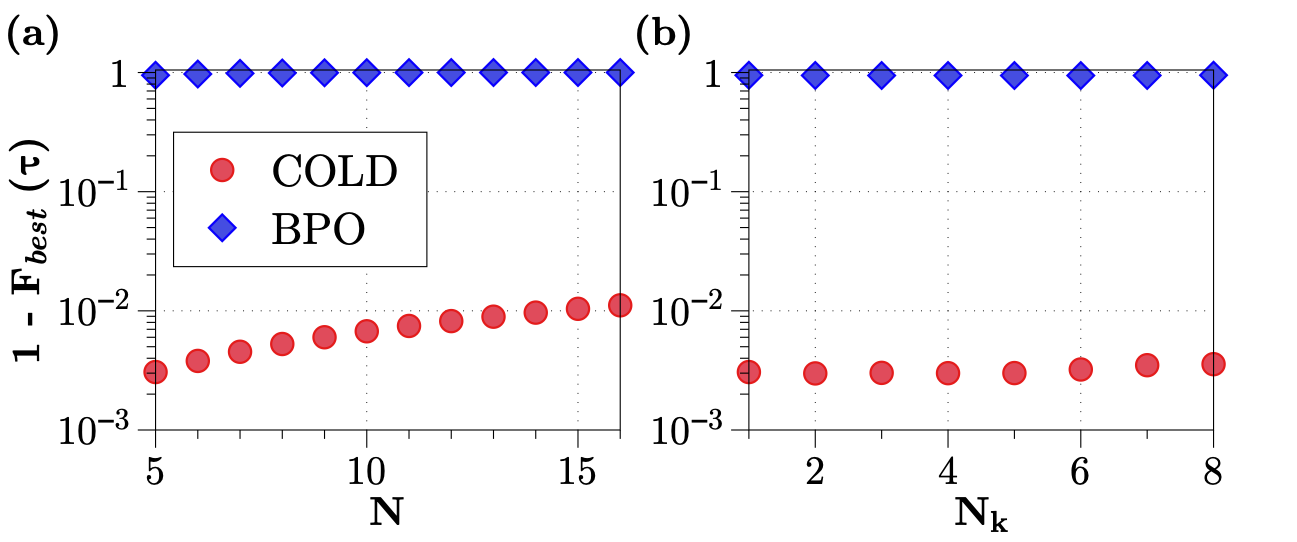
\includegraphics[width=\linewidth]{images/ScalingN.png} \caption[Plots of how final state fidelities scale using COLD and BPO for different system sizes and optimisable parameters.]{Scaling of fidelities in the annealing protocol for the Ising model with (a) system size $N$ and (b) optimisation parameters $N_k$ at driving time $\tau=10^{-2}J_0^{-1}$. Plots show a comparison between \acrref{BPO} (blue diamonds) and \acrref{COLD} (red circles). Plotted best fidelities are obtained across 500 optimisations. Reprinted with permission from \cite{cepaite_counterdiabatic_2023}. Copyright 2023, American Physical Society.}\label{fig:ising_scalingN}
\end{figure}

In Fig.~\ref{fig:ising_maxamp}, we plot the scaling of the \acrref{FO} and \acrref{SO} counterdiabatic terms applied to the five spin Ising chain from Eq.~\eqref{eq:ising_fo_agp} and Eq.~\eqref{eq:ising_so_lcd_terms} with the $\dotlambda$ term included, \@i.e. for the coefficient $\alpha$ we plot the exact \acrref{CD} amplitude of the given \acrref{LCD} operator $\dotlambda \alpha$. In (a) we see the how the different \acrref{LCD} drive amplitudes scale with increasing driving time and in (b) we do the same in the case of the optimised pulses for \acrref{COLD} which were used to obtain the fidelities in Fig.~\ref{fig:ising_unconstrained}(a). Note that while we plot the \acrref{SO} terms for both cases, these were not actually implemented in obtaining the fidelities plotted in the main text. We find, as expected based on the included $\dotlambda$ scaling, that the \acrref{LCD} coefficients decrease linearly with respect to the driving time $\tau$ due to the fact that $\dotlambda = \frac{1}{\tau}$. The coefficients $\alpha$, $\gamma$ and $\zeta$, as expected, stay constant due to their lack of dependence on $\tau$. We see that the \acrref{SO} term $\gamma$ is over an order of magnitude larger than either the \acrref{FO} term $\alpha$ or the other \acrref{SO} term $\zeta$. In (b), however, we find that the \acrref{FO} term $\alpha$ dominates the maximal amplitude for all driving times $\tau$. Furthermore, there is no longer a clean, linear dependence of the counterdiabatic coefficients on driving time, as they are now functions of the control pulse which is optimised for a different set of control parameter values at each driving time $\tau$. The inversion in the strength of the \acrref{SO} and \acrref{FO} \acrref{LCD} terms between the \acrref{COLD} and control-free case shows that in this case \acrref{COLD} implements a dynamical Hamiltonain which is favourable for the applied LCD operators, which are local $\sy$ operators on each spin. This behaviour lends support to the ideas presented in Ch.~\ref{chap:5_cd_as_costfunc} as well as the results in Sec.~\ref{sec:7.2_ising_ho_lcd}, wherein properties of the \acrref{LCD} coefficients are used to optimise the Hamiltonian control pulse.

\begin{figure}[t!]
    \centering
    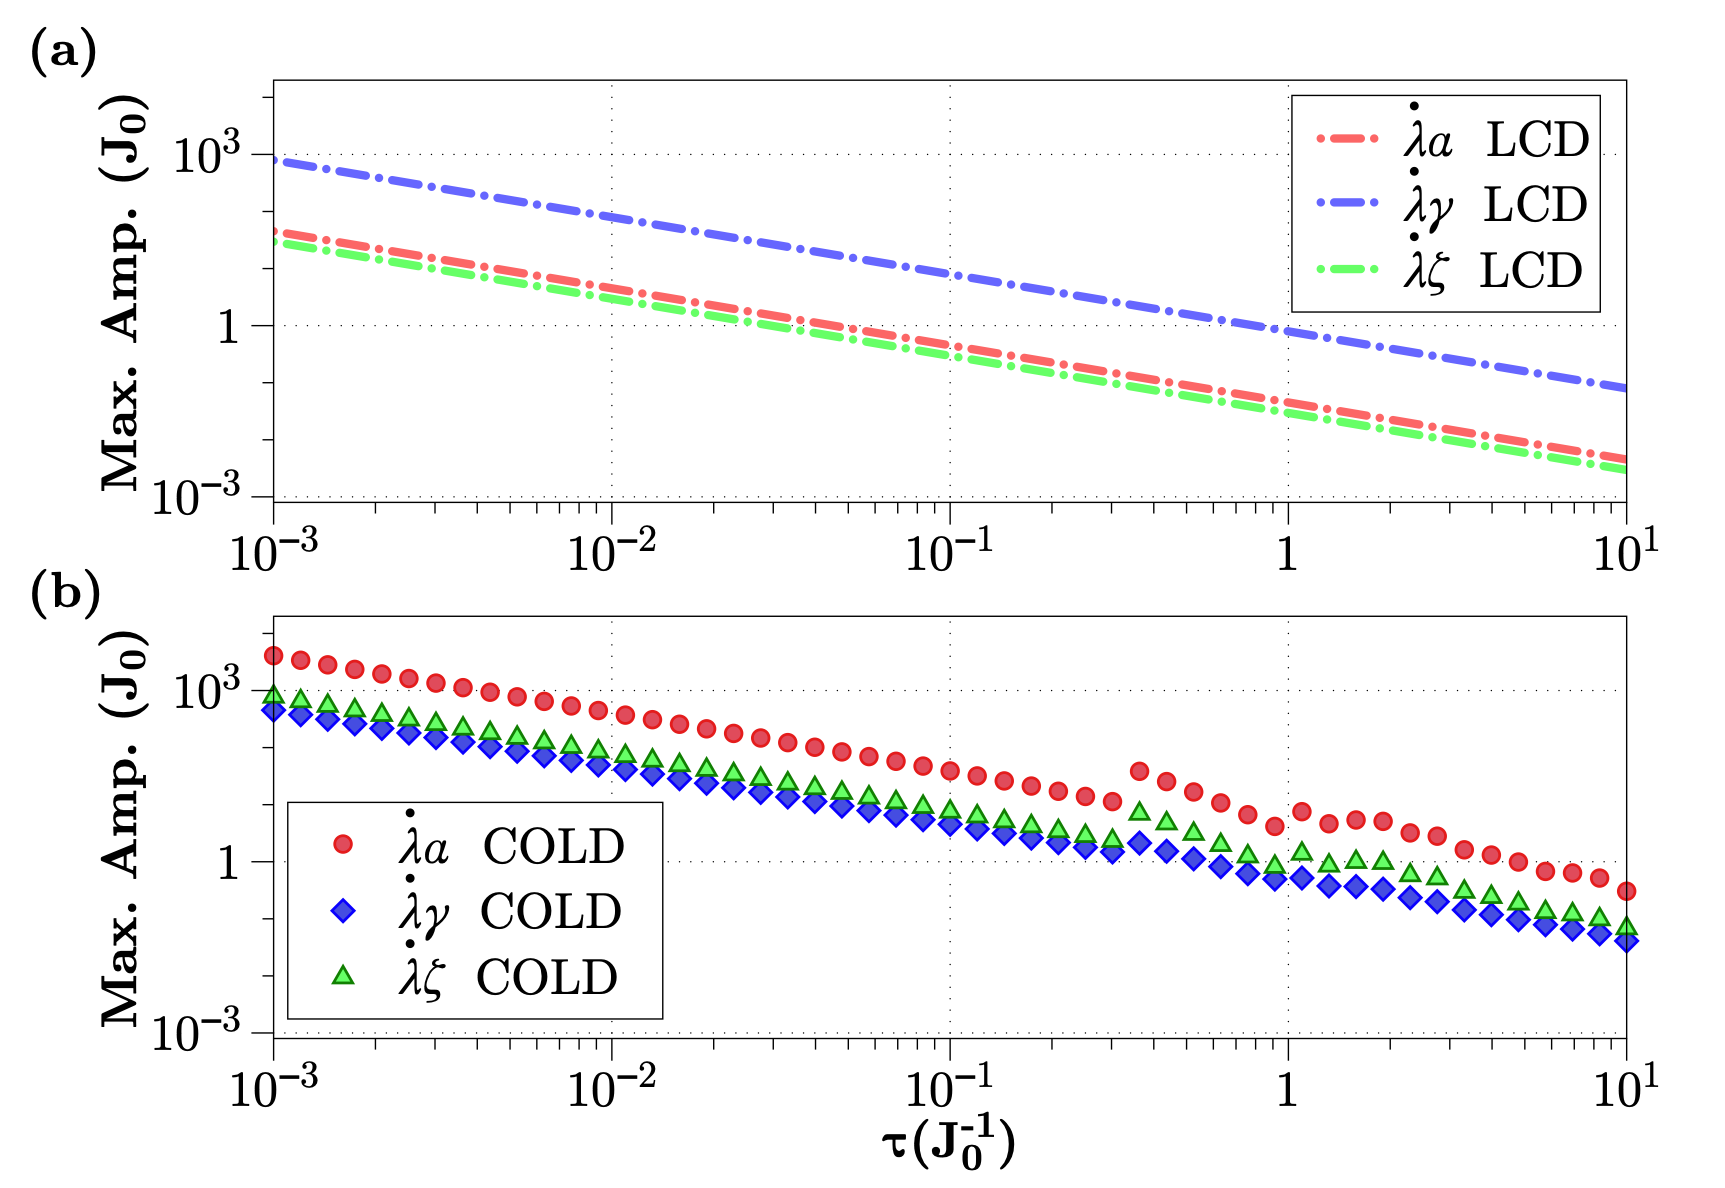
\includegraphics[width=\linewidth]{images/MaxAmp.png} \caption[Plots of maximum amplitudes of LCD drives for the Ising spin chain.]{Maximum amplitudes of \acrref{LCD} terms in the Ising model annealing protocol for (a) \acrref{FO} and \acrref{SO} \acrref{LCD} with no additional optimal control fields and (b) the \acrref{COLD} approach optimised for the best final state fidelity implementing \acrref{FO} LCD as shown in Fig.~\ref{fig:ising_unconstrained}(a). The plot shows the maximum amplitude reached at any point in the drive for different driving times $\tau$ in the case of \acrref{FO} terms $\alpha$ (red circles) and \acrref{SO} terms $\gamma$ (blue diamonds) and $\zeta$ in the case when only the \acrref{FO} terms are applied to the system. Reprinted with changes with permission from \cite{cepaite_counterdiabatic_2023}. Copyright 2023, American Physical Society.}\label{fig:ising_maxamp}
\end{figure}

\chapter{Additional plots on GHZ state preparation using AGP as a cost function}\label{app:higher_order_AGP}

In Sec.~\ref{sec:7.3_ghz_ho}, we considered using \acrref{AGP}-based cost functions, which were introduced in detail in Ch.~\ref{chap:5_cd_as_costfunc}, in GHZ state preparation in a system of $N=3$ frustrated spins. We found that, when using a control pulse constructed from \acrref{GRAPE}, there appears to be no advantage to using \acrref{FO} or \acrref{SO} \acrref{LCD} information in the optimisation process, whether integrals or maximum amplitudes of the operator coefficients. In Fig.~\ref{fig:ghz_contours} in the main text, we plotted the cost function landscapes of the fidelity cost function $C_{\rm F}$, the tangle cost function $C_{T_3}$ and several integral cost functions $C_{\rm I}$ in the case of different \acrref{LCD} coefficients for total driving time $\tau = 0.1J_0^{-1}$ and for two control parameters $c_1, c_2 \in [-10,10]$. The results showed a highly non-convex landscape with respect to the final state fidelity and the three-tangle, which measures the amount of GHZ-type entanglement in a system. There also appeared to be no significant correlation between the minimum and maximum values of the integral cost functions and the quality of the final state, \@i.e.~either the final state fidelity or the amount of entanglement in the final state. 

\begin{figure}[t!]
    \centering
    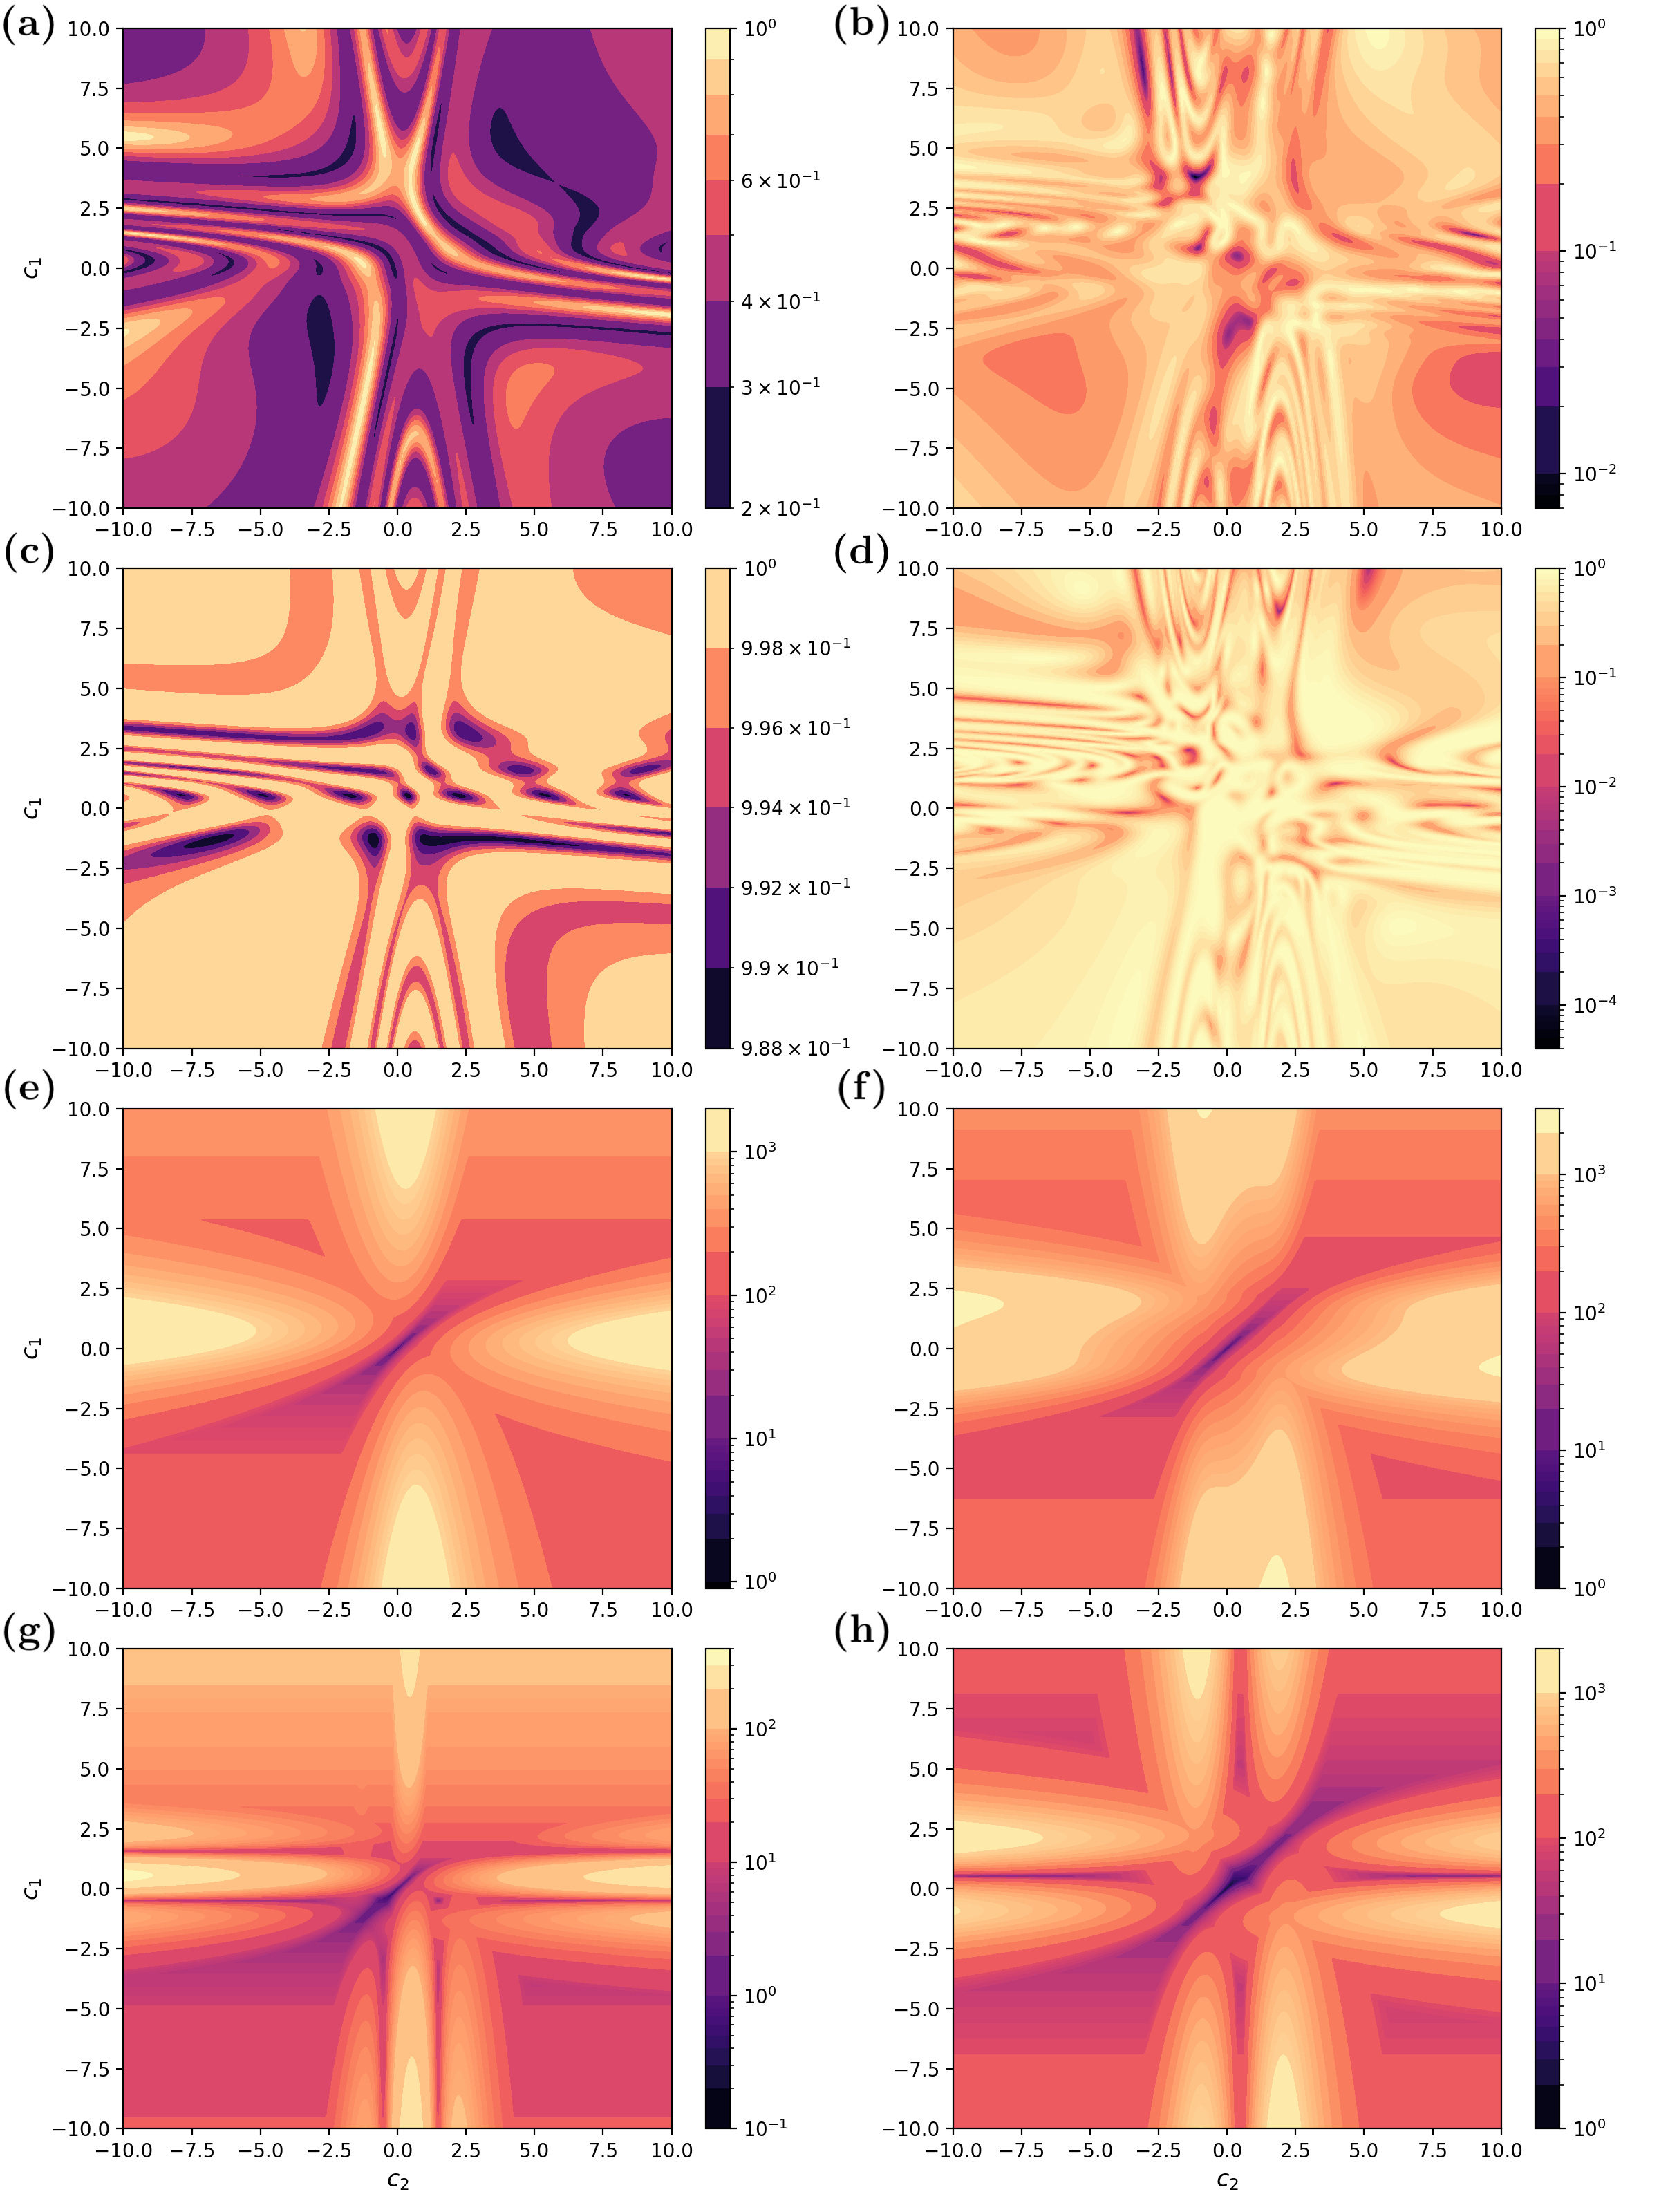
\includegraphics[width=0.8\linewidth]{images/ghz_contour_maximums.png} \caption[Contour plots of cost function landscapes for GHZ state preparation in frustrated spin systems (maximum amplitude cost function).]{Contour plots at $\tau = 0.1 J_0^{-1}$ of different cost function values for GHZ state preparation for parameters $c_1, c_2 \in [-10,10]$ and a \acrref{GRAPE} control pulse. In (a) and (b) we plot $C_{\rm F}$ in the cases where \acrref{FO} and \acrref{SO} \acrref{COLD} is applied respectively. Then, in (c-d) we do the same for $C_{T_3}$, with \acrref{FO} \acrref{COLD} plotted in (c) and \acrref{SO} \acrref{COLD} plotted in (d). (e-h) are then plots of the maximum amplitude cost function $C_{\rm A}$ values for the same range of parameters. In (e) we plot $C_{\rm A, \alpha^{(1)}}$ when only \acrref{FO} \acrref{LCD} is considered, while in (f) we plot $C_{\rm A, \alpha^{(2)}}$ as described in the text. Then in (g) we plot $C_{\rm A, \gamma}$ and in (h) we plot $C_{\rm a, \zeta}$, corresponding to the \acrref{SO} terms. Note that each plot has its own color bar, as the color encodings and the value scaling in each plot is quite different.} \label{fig:ghz_contours_max_appendix}
\end{figure}

In Fig.~\ref{fig:ghz_contours_max_appendix} we reproduce the landscapes of $C_{\rm F}$ and $C_{T_3}$ from Fig.~\ref{fig:ghz_contours} and then plot the results for the maximum amplitude cost function $C_{\rm A}$ in plots (e-h) corresponding to the same coefficients as were plotted for the integral cost function in the main text. While there is some minimal difference in the landscapes between $C_{\rm I}$ and $C_{\rm A}$, they broadly follow similar trends and show no correlation with fidelity or entanglement.

To be sure that this failure is not a consequence of constructing the control pulse using the \acrref{GRAPE} algorithm, we also implement a bare control pulse like that described in Eq.~\eqref{eq:ising_control_nocrab} and plot the results in Fig.~\ref{fig:ghz_contours_max_noGRAPE} for the maximum amplitude cost functions $C_{\rm A}$ as well as integral cost functions $C_{\rm I}$ in Fig.~\ref{fig:ghz_contours_int_noGRAPE}. While the cost function landscapes are far smoother, the resulting fidelities and entanglement in the final state are orders of magnitude worse than those using the \acrref{GRAPE} pulse. Furthermore, there once again does not appear to be any advantage to using the \acrref{AGP}-based cost functions. The maximum entanglement (in the given range of parameters) when applying \acrref{SO} terms, for example, as shown in Fig.~\ref{fig:ghz_contours_max_noGRAPE}(d), occurs close to the minimum of the \acrref{SO} pulse integrals and maximal amplitudes (plots (g-h) in Fig.~\ref{fig:ghz_contours_max_noGRAPE} and plots (c-d) in Fig.~\ref{fig:ghz_contours_int_noGRAPE}, which is not what we would expect based on the conjecture that an optimal pulse would maximise the effects of the \acrref{LCD} operators that are being applied. Any attempts at optimisation using $C_{\rm I}$ or $C_{\rm A}$ pulses does not return better results than in the \acrref{GRAPE} case.

\begin{figure}[t!]
    \centering
    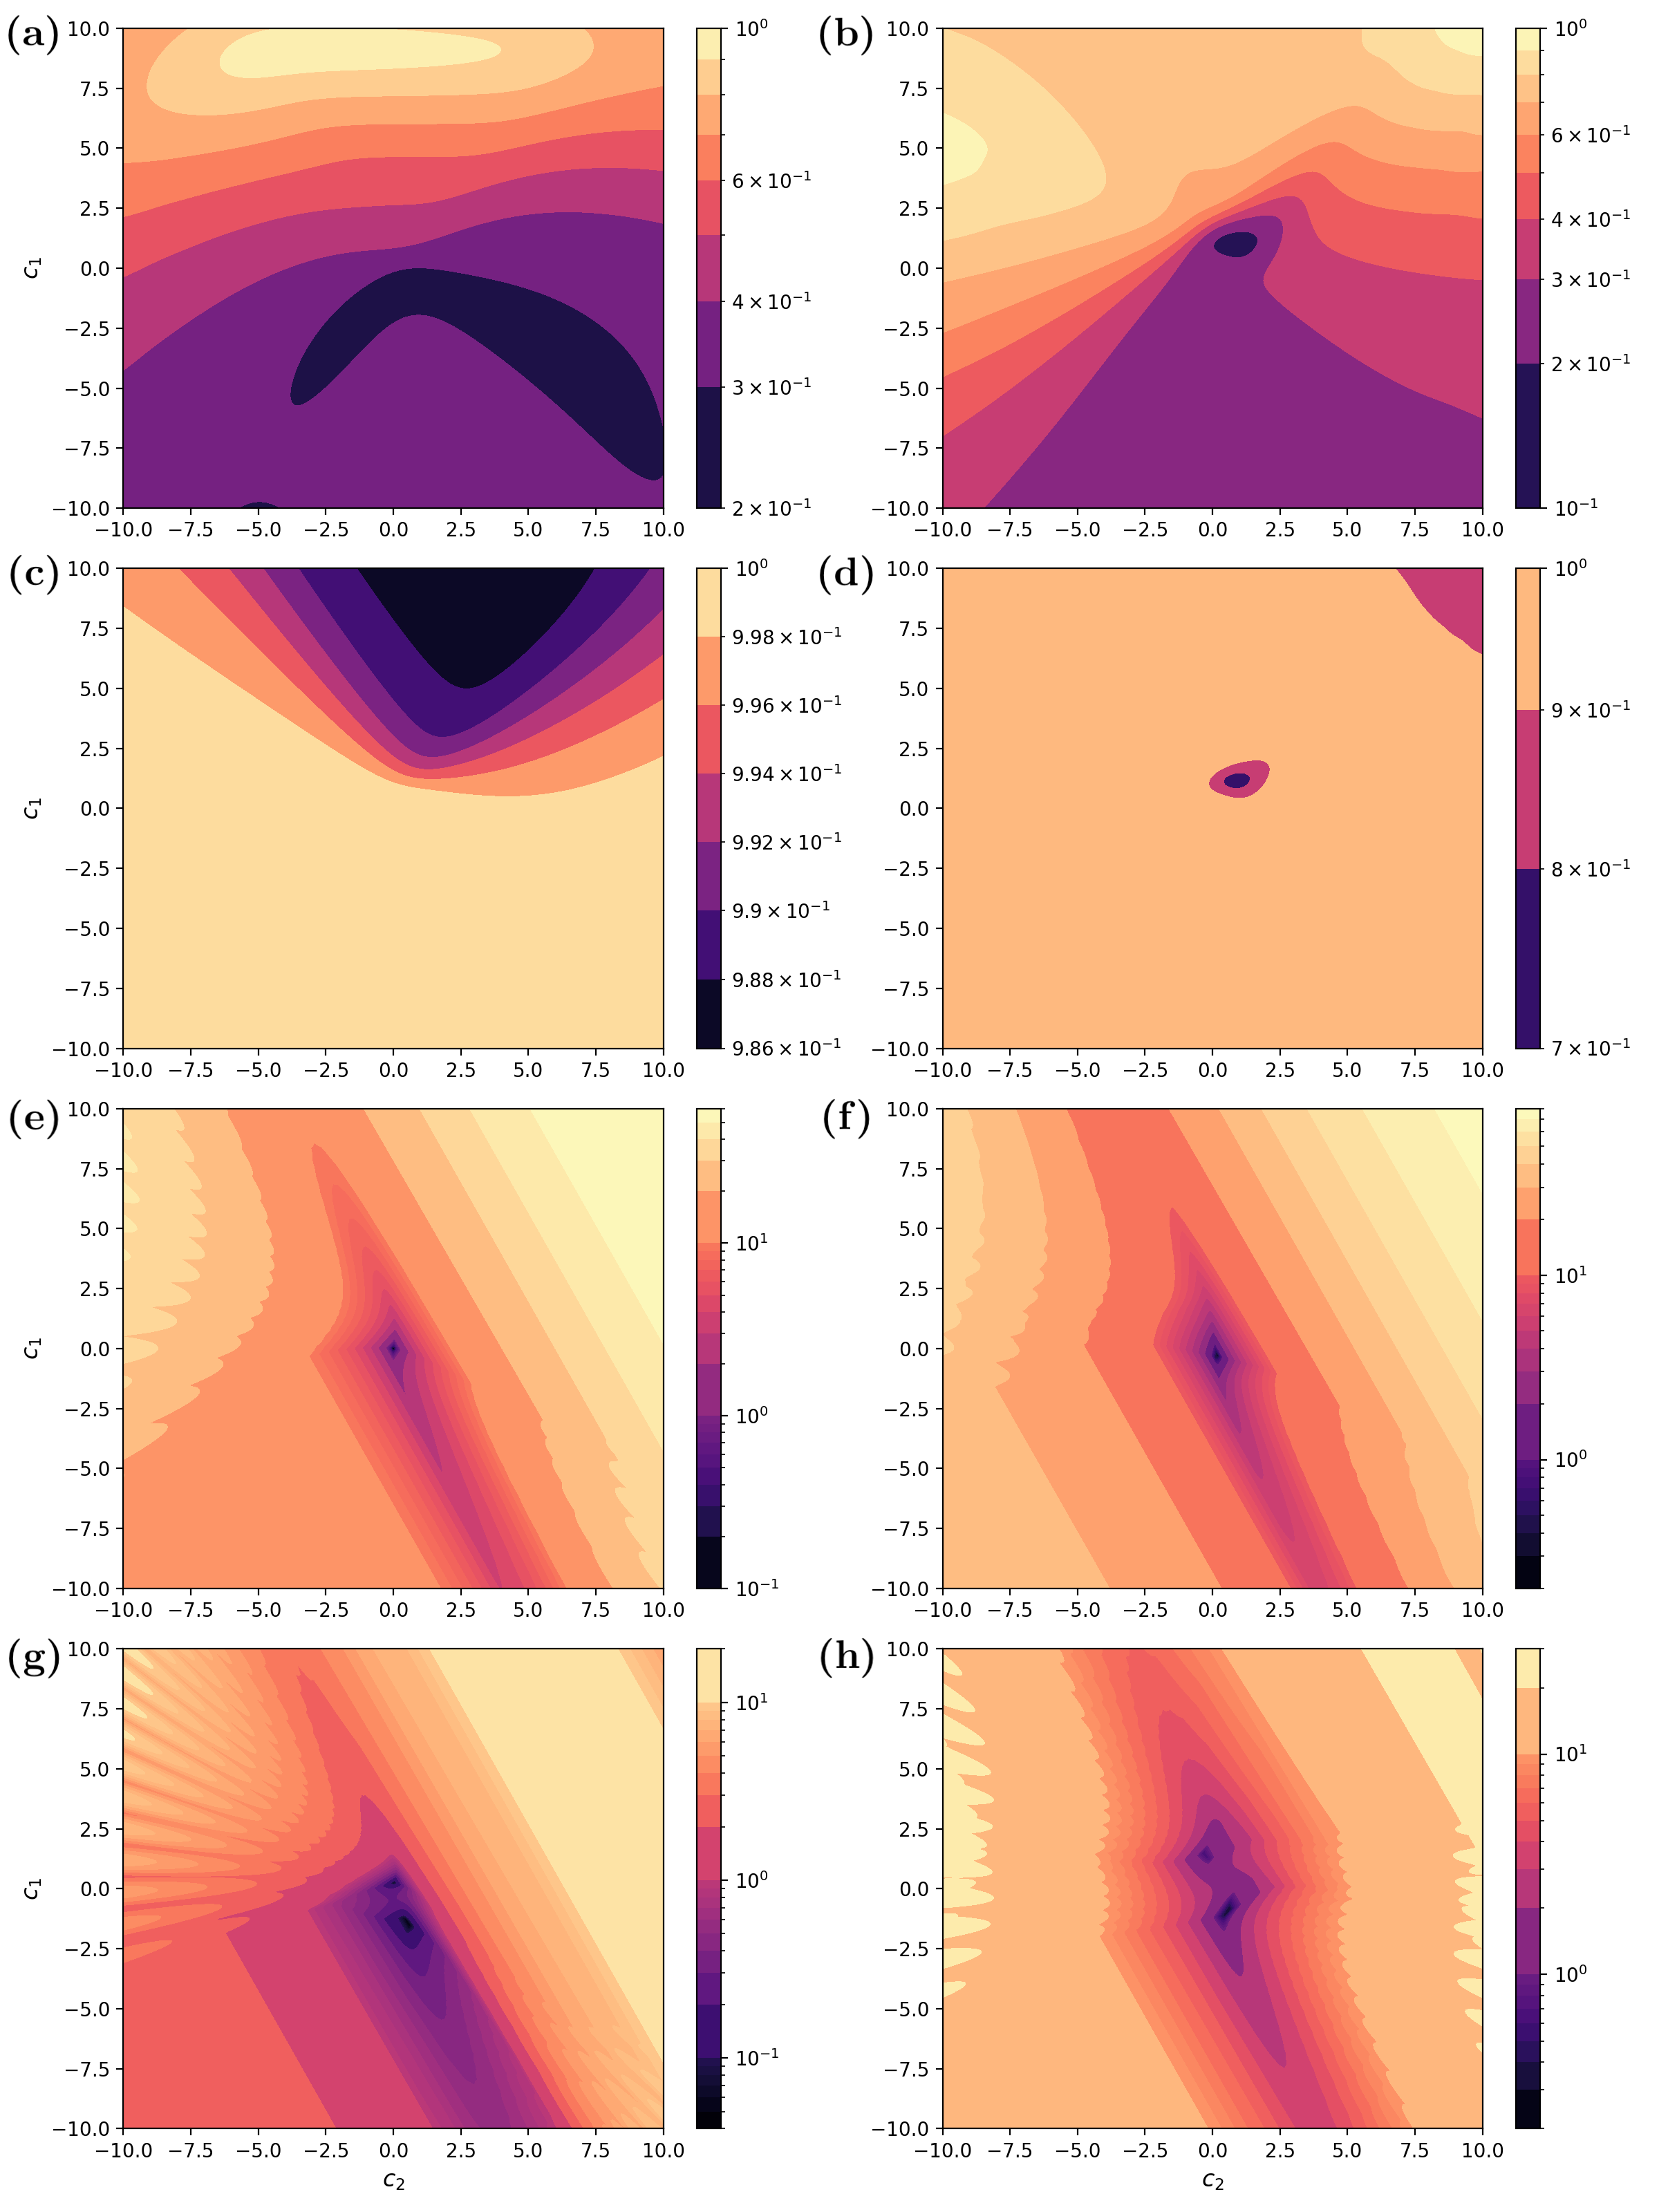
\includegraphics[width=0.8\linewidth]{images/final_plot_max_nogrape.png} \caption[Contour plots of cost function landscapes for GHZ state preparation in frustrated spin systems (maximum amplitude cost function) using a bare optimisation pulse.]{Contour plots at $\tau = 0.1 J_0^{-1}$ of different cost function values for GHZ state preparation for parameters $c_1, c_2 \in [-10,10]$ and a bare control pulse. In (a) and (b) we plot $C_{\rm F}$ in the cases where \acrref{FO} and \acrref{SO} \acrref{COLD} is applied respectively. Then, in (c-d) we do the same for $C_{T_3}$, with \acrref{FO} \acrref{COLD} plotted in (c) and \acrref{SO} \acrref{COLD} plotted in (d). (e-h) are then plots of the maximum amplitude cost function $C_{\rm A}$ values for the same range of parameters. In (e) we plot $C_{\rm A, \alpha^{(1)}}$ when only \acrref{FO} \acrref{LCD} is considered, while in (f) we plot $C_{\rm A, \alpha^{(2)}}$ as described in the text. Then in (g) we plot $C_{\rm A, \gamma}$ and in (h) we plot $C_{\rm A, \zeta}$, corresponding to the \acrref{SO} terms.}\label{fig:ghz_contours_max_noGRAPE}
\end{figure}

\begin{figure}[t!]
    \centering
    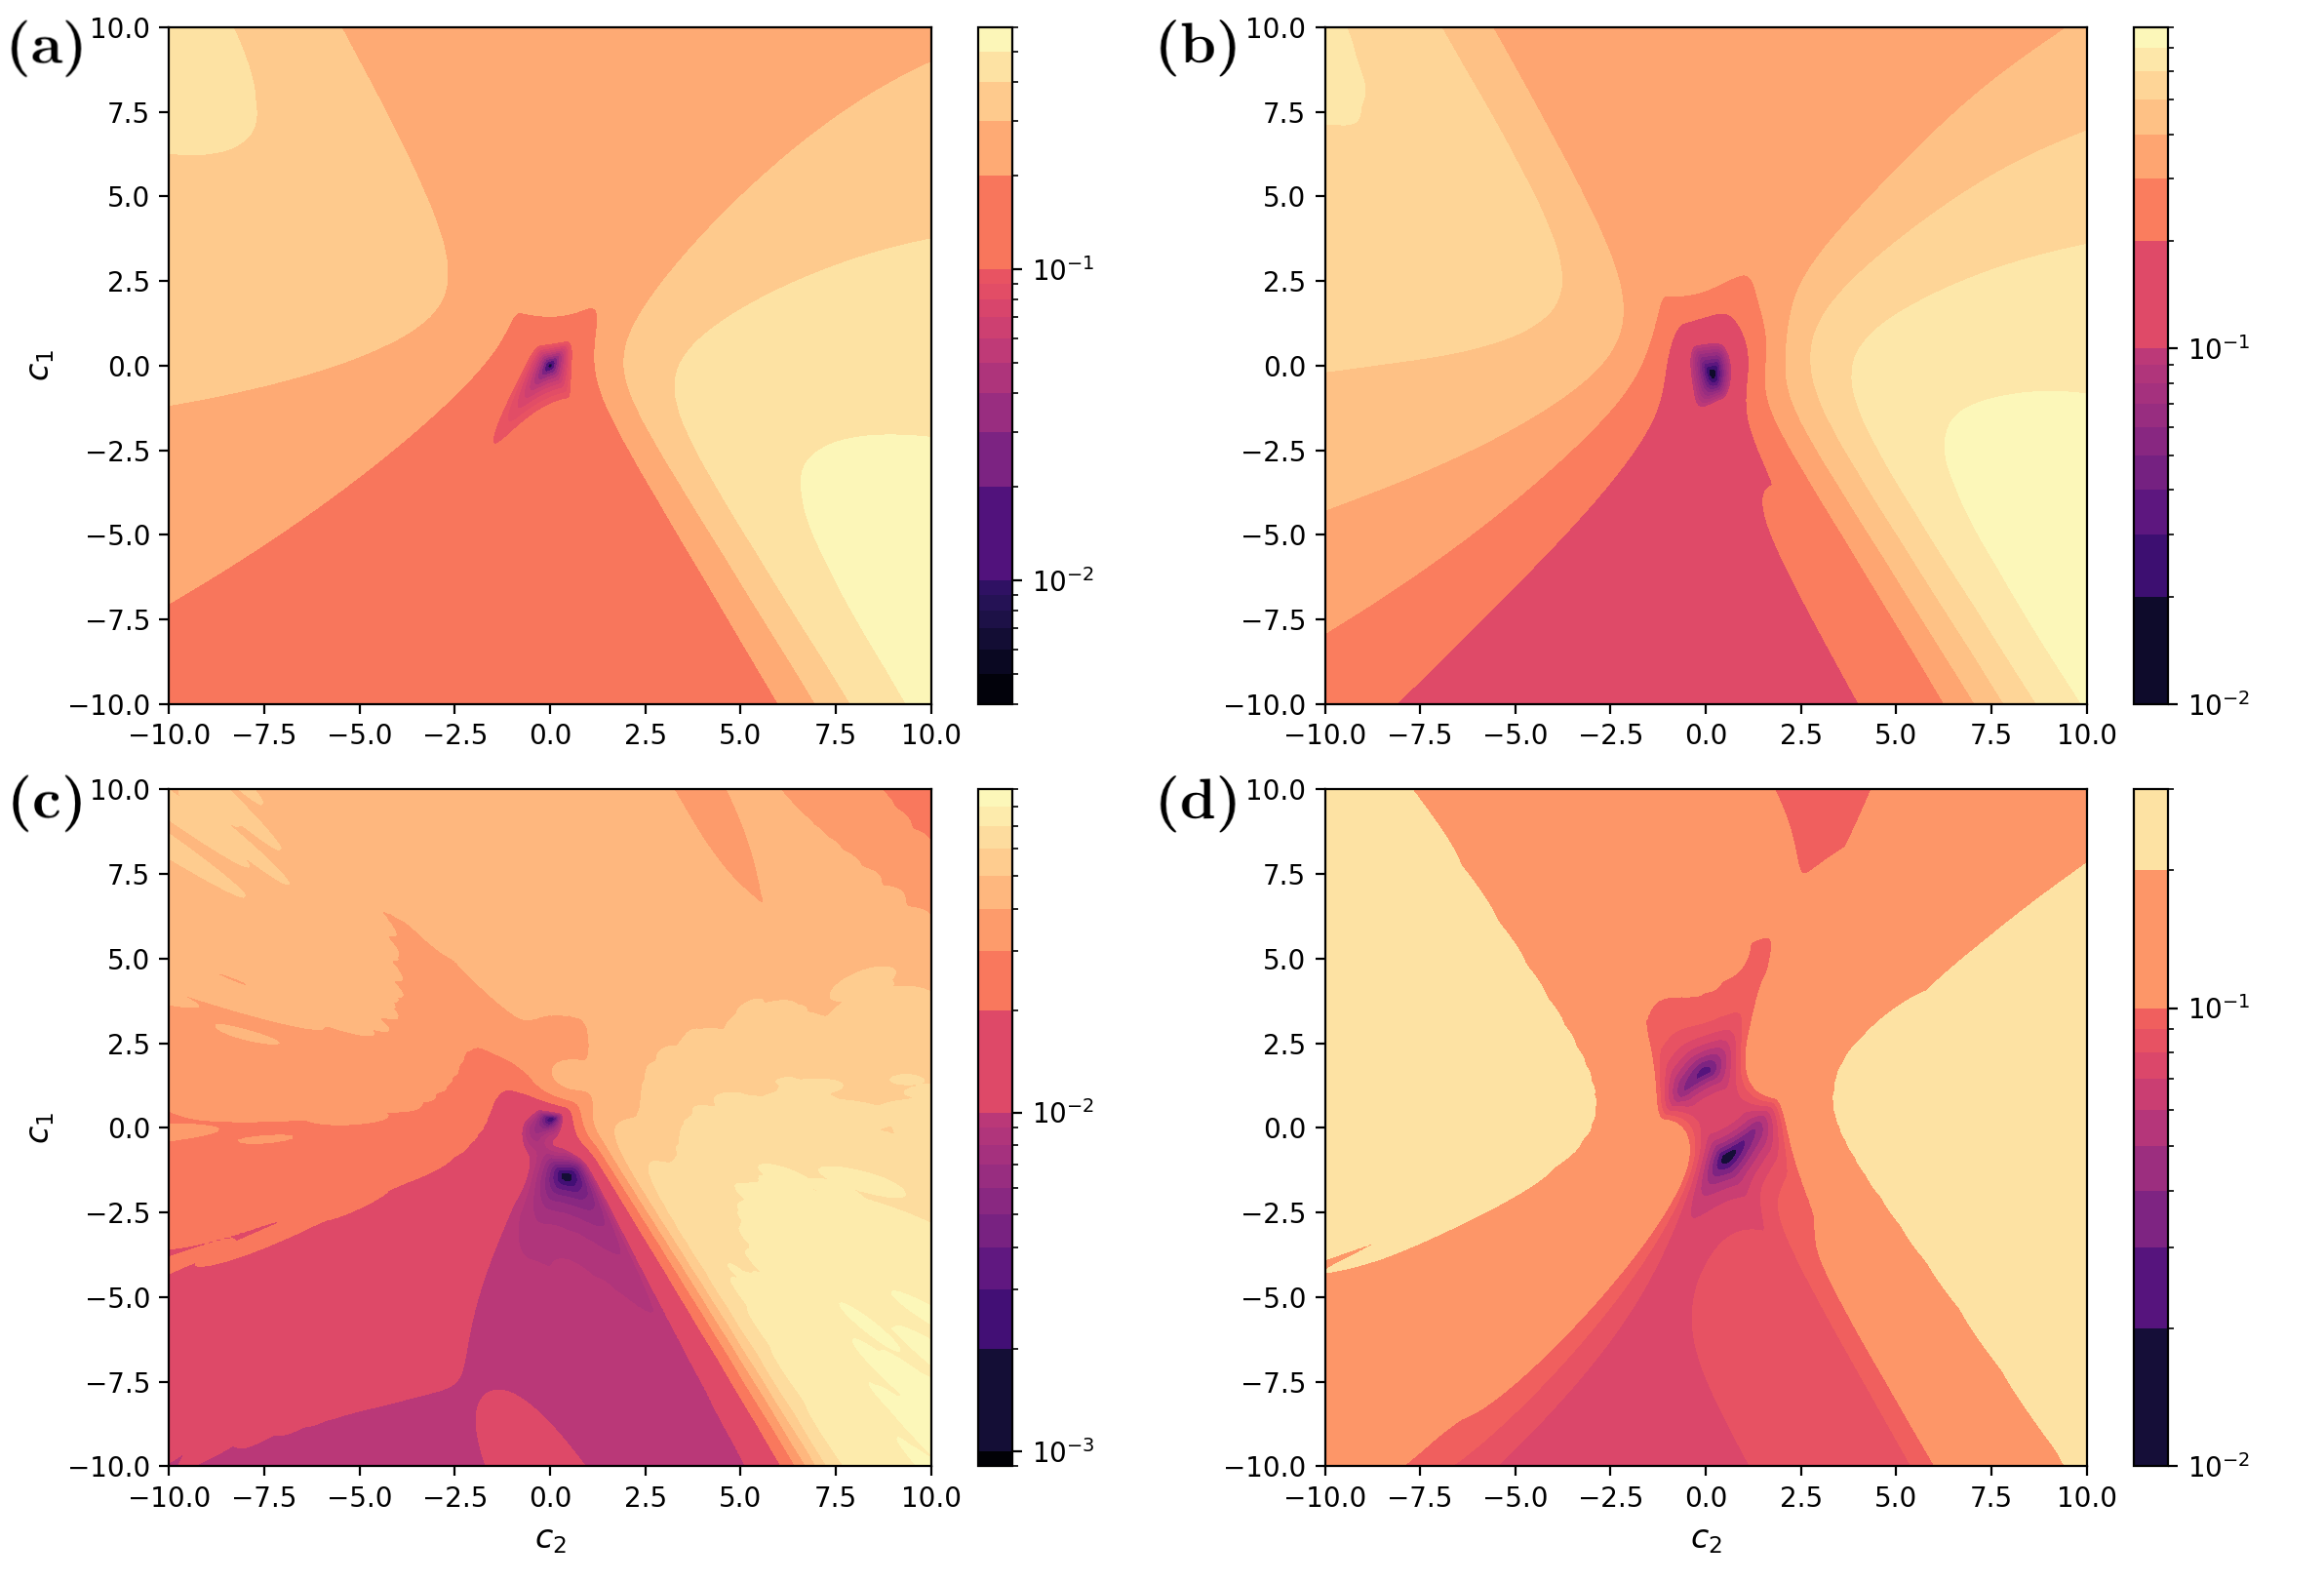
\includegraphics[width=0.9\linewidth]{images/final_plot_int_nogrape.png} \caption[Contour plots of cost function landscapes for GHZ state preparation in frustrated spin systems (integral cost function) using a bare optimisation pulse.]{Contour plots at $\tau = 0.1 J_0^{-1}$ of different cost function values for GHZ state preparation for parameters $c_1, c_2 \in [-10,10]$ and a bare control pulse. In (a) we plot $C_{\rm I, \alpha^{(1)}}$ when only \acrref{FO} \acrref{LCD} is considered, while in (b) we plot $C_{\rm I, \alpha^{(2)}}$ as described in the text. Then in (c) we plot $C_{\rm I, \gamma}$ and in (d) we plot $C_{\rm I, \zeta}$, corresponding to the \acrref{SO} terms.}\label{fig:ghz_contours_int_noGRAPE}
\end{figure}
